\documentclass[11pt, xcolor={dvipsnames}, usepdftitle=false]{beamer}
\usepackage{presentation}
\usepackage[brazil]{babel}
\usepackage[utf8]{inputenc}
\usepackage{graphicx}
\hypersetup{pdfpagemode=UseNone, hidelinks, pdfdisplaydoctitle=true,%
pdftitle={Reserva de Salas -- Apresentação de Banca (versão detalhada)}}

\input{../../../out/drive-links.tex}

\title{Reserva de Salas}
\author{José Ronaldo dos Santos Júnior\\[2mm]{\small Orientador: Prof.\ Gustavo Queiroz Silveira}}
\date{Ciência da Computação -- Centro Universitário Filadélfia\\[1mm]Londrina, Junho de 2026}

\begin{document}
\frame{\titlepage}

% ---- Objetivos e Motivações ----
\begin{frame}
\frametitle{Objetivos e Motivações}
\textbf{Problema:} hoje o gerenciamento de salas é feito de forma manual, em planilhas. Com a alta demanda, as trocas de horário e as restrições de uso, o processo se torna complexo.
\begin{itemize}
\item Conflitos de agendamento
\item Retrabalho no controle das reservas
\item Perda de rastreabilidade de quem reservou o quê
\end{itemize}
\vspace{2mm}
\textbf{Objetivo principal:} desenvolver uma solução de agendamento de salas para a UniFil.
\begin{itemize}
\item Centralizar as informações de agendamento em um só lugar
\item Automatizar o fluxo de solicitação e aprovação de reservas
\item Manter um histórico das alterações
\end{itemize}
\end{frame}

% ---- Tecnologias ----
\begin{frame}
\frametitle{Tecnologias Utilizadas}
\begin{itemize}
\item \textbf{Linguagens de Programação:}
\begin{itemize}
\item \textit{Back-end}: Java --- ecossistema consolidado no mercado corporativo
\item \textit{Front-end}: JavaScript --- padrão para interfaces web
\end{itemize}
\item \textbf{Banco de Dados:} PostgreSQL --- maturidade e boa integração com os frameworks adotados
\item \textbf{Frameworks de Desenvolvimento:}
\begin{itemize}
\item \textit{Front-end}: React --- interface reativa e componentizada
\item \textit{Back-end}: Spring Boot --- exposição de uma API REST sobre o ecossistema Spring
\end{itemize}
\end{itemize}
\end{frame}

% ---- Separador: Diagramas ----
\begin{frame}
\heading{Diagramas}
\end{frame}

% ---- Workflow AS-IS ----
\begin{frame}
\frametitle{Workflow AS-IS (BPMN)}
{\footnotesize Mapeamento do processo atual: o professor consulta a planilha manualmente; conflitos de horário são resolvidos por negociação informal; e a aprovação do coordenador termina em atualização manual da planilha. É manual nos pontos críticos.}
\begin{figure}
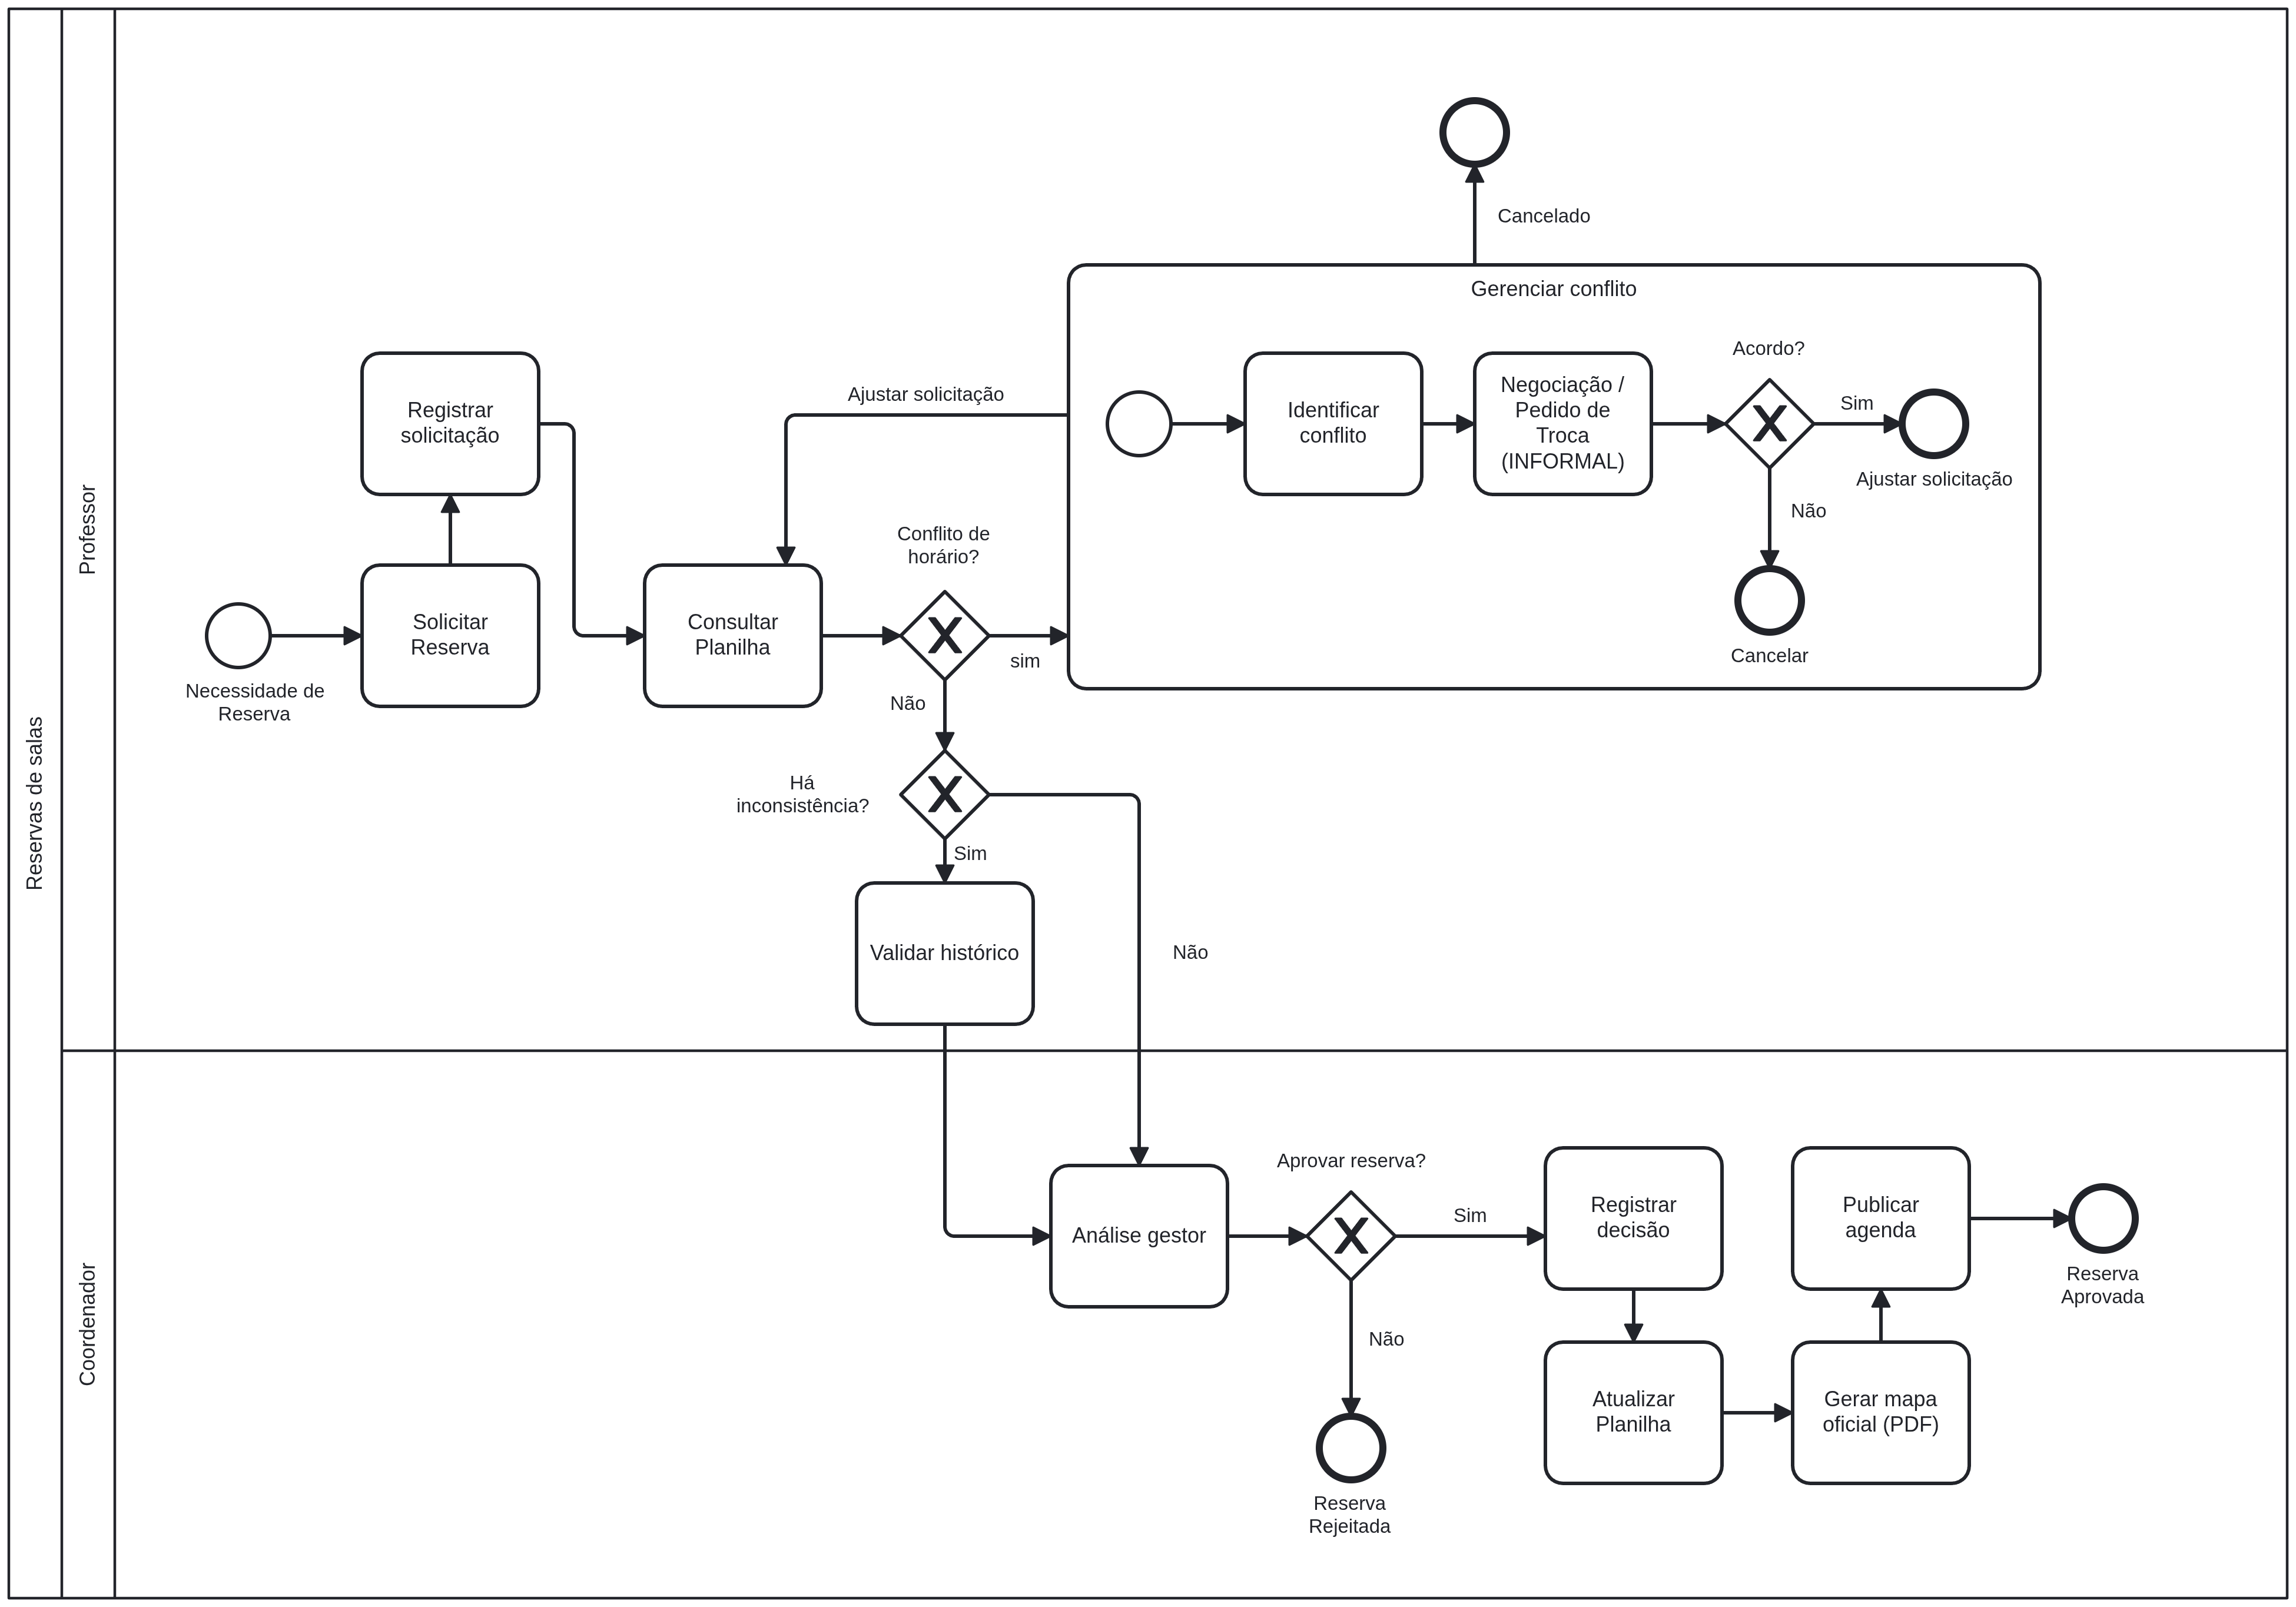
\includegraphics[width=\textwidth,height=0.6\textheight,keepaspectratio]{../relatorio-estagio/imagens/workflow-as-is.png}
\end{figure}
\end{frame}

% ---- Diagrama de Caso de Uso ----
\begin{frame}
\frametitle{Diagrama de Caso de Uso}
{\footnotesize A partir do processo, foram levantados os casos de uso: autenticação, gerenciamento de salas e de seus recursos, fluxo de agendamento, histórico e relatórios.}
\begin{figure}
\includegraphics[width=\textwidth,height=0.62\textheight,keepaspectratio]{../../../out/src/plantuml/usecasediagram.png}
\end{figure}
\end{frame}

% ---- Atores ----
\begin{frame}
\frametitle{Atores do Sistema}
\begin{itemize}
\item \textbf{sa\_professor} --- usuário comum do sistema:
\begin{itemize}
\item Autenticação, gerenciamento de salas e agendamentos
\item Geração de relatórios e consulta ao histórico
\end{itemize}
\item \textbf{sa\_coordenador} --- especialização de \textbf{sa\_professor}:
\begin{itemize}
\item Herda todas as permissões do professor
\item Ganha, adicionalmente, o acesso ao gerenciamento de usuários
\end{itemize}
\end{itemize}
\end{frame}

% ---- DER ----
\begin{frame}
\frametitle{Modelagem do Banco de Dados (DER)}
{\footnotesize Modelagem das entidades no banco. As centrais são usuário, sala, tipo de sala, recurso e prédio, além das entidades de agendamento. As relações garantem, por exemplo, que cada sala pertence a um prédio e a um tipo, e que uma sala pode ter vários recursos.}
\begin{figure}
\includegraphics[width=\textwidth,height=0.62\textheight,keepaspectratio]{../../../out/src/plantuml/der-horizontal.png}
\end{figure}
\end{frame}

% ---- Diagrama de Componentes ----
\begin{frame}
\frametitle{Diagrama de Componentes: Visão Geral dos Módulos}
\begin{columns}[c]
\begin{column}{0.44\textwidth}
\small
O sistema é organizado em módulos por domínio: autenticação, usuários, salas e eventos.
\vspace{3mm}

A comunicação entre eles é controlada:
\begin{itemize}
\item autenticação acessa usuários por uma porta bem definida;
\item eventos referenciam usuário e sala apenas pelo identificador.
\end{itemize}
\vspace{2mm}
Isso mantém as fronteiras entre os módulos claras.
\end{column}
\begin{column}{0.56\textwidth}
\includegraphics[width=\textwidth,height=0.8\textheight,keepaspectratio]{../../../out/src/plantuml/componentes.png}
\end{column}
\end{columns}
\end{frame}

% ---- Diagramas de Classes ----
\begin{frame}
\frametitle{Diagrama de Classe --- Usuário}
{\footnotesize Estrutura em camadas: domínio no centro (entidade \texttt{User}), aplicação com os casos de uso (criar, atualizar) e infraestrutura por fora (controller e repositório).}
\begin{figure}
\includegraphics[width=\textwidth,height=0.62\textheight,keepaspectratio]{../../../out/src/plantuml/classe/user.png}
\end{figure}
\end{frame}

\begin{frame}
\frametitle{Diagrama de Classe --- Sala}
\begin{figure}
\includegraphics[width=\textwidth,height=0.62\textheight,keepaspectratio]{../../../out/src/plantuml/classe/room.png}
\end{figure}
\end{frame}

\begin{frame}
\frametitle{Diagrama de Classe --- Evento}
\begin{figure}
\includegraphics[width=\textwidth,height=0.62\textheight,keepaspectratio]{../../../out/src/plantuml/classe/event.png}
\end{figure}
\end{frame}

\begin{frame}
\frametitle{Diagrama de Classe --- Autenticação}
\begin{figure}
\includegraphics[width=\textwidth,height=0.62\textheight,keepaspectratio]{../../../out/src/plantuml/classe/auth.png}
\end{figure}
\end{frame}

% ---- Diagrama de Estado: Usuário ----
\begin{frame}
\frametitle{Diagrama de Estado --- Usuário}
{\footnotesize Entidades com ciclo de vida controlado por estados. O usuário transita entre ativo, inativo e excluído, e cada transição é uma operação específica do sistema, não uma edição livre do campo, o que evita estados inválidos.}
\begin{figure}
\includegraphics[width=\textwidth,height=0.6\textheight,keepaspectratio]{../../../out/src/plantuml/estado/user_status.png}
\end{figure}
\end{frame}

% ---- Diagramas de Sequência: Usuário e Sala (representativos) ----
\begin{frame}
\frametitle{Diagrama de Sequência --- Criar Usuário}
{\footnotesize Colaboração das camadas em tempo de execução: a requisição chega no controller, vai para o caso de uso, que cria a entidade e a persiste pelo repositório, devolvendo a resposta. Cada camada com responsabilidade clara.}
\begin{figure}
\includegraphics[width=\textwidth,height=0.6\textheight,keepaspectratio]{../../../out/src/plantuml/sequencia/user/create_user.png}
\end{figure}
\end{frame}

\begin{frame}
\frametitle{Diagrama de Sequência --- Criar Sala}
\begin{figure}
\includegraphics[width=\textwidth,height=0.6\textheight,keepaspectratio]{../../../out/src/plantuml/sequencia/room/create_room.png}
\end{figure}
\end{frame}

% ---- Diagrama de Implantação ----
\begin{frame}
\frametitle{Diagrama de Implantação}
{\footnotesize Arquitetura separada por responsabilidades: o navegador do cliente acessa o front-end, que conversa com a API do back-end por HTTPS, e a API acessa o banco PostgreSQL.}
\begin{figure}
\includegraphics[width=\textwidth,height=0.62\textheight,keepaspectratio]{../../../out/src/plantuml/deployment.png}
\end{figure}
\end{frame}

% ---- Separador: Telas ----
\begin{frame}
\heading{Apresentação do Sistema}
\end{frame}

% ---- Transição para demonstração ao vivo ----
\begin{frame}
\frametitle{Demonstração}
A seguir, demonstração ao vivo do sistema, percorrendo o núcleo do que já está funcionando:
\begin{itemize}
\item Login e autenticação
\item Cadastro e gerenciamento de salas (tipo, capacidade e recursos)
\item Busca de salas disponíveis
\item Solicitação e acompanhamento de reservas
\item Grade de horários e ocupação das salas
\end{itemize}
\vspace{3mm}
\end{frame}

% ---- Artefatos de Requisitos ----
\begin{frame}
\frametitle{Artefatos de Requisitos}
\begin{itemize}
\item \textbf{Documento de Visão}
\item \textbf{Especificação Complementar}
\item \textbf{Glossário}
\item \textbf{Solicitação dos Principais Envolvidos}
\item \textbf{Especificação de Caso de Uso}
\end{itemize}
\end{frame}

% ---- Conceitos de Engenharia de Software Aplicados ----
\begin{frame}
\frametitle{Conceitos de Engenharia de Software Aplicados}
Um objetivo do estágio foi aplicar, na prática, conceitos de engenharia de software:
\begin{itemize}
\item \textbf{Clean Architecture (Ports \& Adapters):} domínio, aplicação e infraestrutura separados; portas implementadas por adaptadores
\item \textbf{Domain-Driven Design:} entidades ricas em comportamento, value objects para os identificadores e agregados referenciados por ID
\item \textbf{Notification Pattern:} validações que acumulam os erros, em vez de estourar exceção campo a campo
\item \textbf{Monólito Modular:} módulos por domínio com núcleo compartilhado, comunicando-se via portas
\end{itemize}
\end{frame}

% ---- Conclusão ----
\begin{frame}
\frametitle{Conclusão}
\textbf{Resultados alcançados:}
\begin{itemize}
\item Autenticação e gerenciamento de usuários (professor/coordenador)
\item Cadastro e gerenciamento de salas, recursos e prédios
\item Modelagem completa do sistema (casos de uso, DER, classes, sequência, implantação)
\end{itemize}
\vspace{3mm}
\textbf{Em desenvolvimento:}
\begin{itemize}
\item Fluxo de solicitação e aprovação de reservas
\item Grade de horários e visualização de disponibilidade
\end{itemize}
\end{frame}

% ======================================================================
% Slides de apoio (não apresentados no tempo principal; usar se a banca
% perguntar sobre algum desses diagramas/entidades específicas)
% ======================================================================

\begin{frame}
\heading{Slides de Apoio}
\end{frame}

\begin{frame}
\frametitle{Diagrama de Estado --- Sala}
\begin{figure}
\includegraphics[width=\textwidth,height=0.7\textheight,keepaspectratio]{../../../out/src/plantuml/estado/room_status.png}
\end{figure}
\end{frame}

\begin{frame}
\frametitle{Diagrama de Estado --- Tipo de Sala}
\begin{figure}
\includegraphics[width=\textwidth,height=0.7\textheight,keepaspectratio]{../../../out/src/plantuml/estado/room_type_status.png}
\end{figure}
\end{frame}

\begin{frame}
\frametitle{Diagrama de Estado --- Prédio}
\begin{figure}
\includegraphics[width=\textwidth,height=0.7\textheight,keepaspectratio]{../../../out/src/plantuml/estado/building_status.png}
\end{figure}
\end{frame}

\begin{frame}
\frametitle{Diagrama de Estado --- Recurso}
\begin{figure}
\includegraphics[width=\textwidth,height=0.7\textheight,keepaspectratio]{../../../out/src/plantuml/estado/resource_status.png}
\end{figure}
\end{frame}

\begin{frame}
\frametitle{Diagrama de Sequência --- Buscar Usuário}
\begin{figure}
\includegraphics[width=\textwidth,height=0.7\textheight,keepaspectratio]{../../../out/src/plantuml/sequencia/user/get_user.png}
\end{figure}
\end{frame}

\begin{frame}
\frametitle{Diagrama de Sequência --- Atualizar Usuário}
\begin{figure}
\includegraphics[width=\textwidth,height=0.7\textheight,keepaspectratio]{../../../out/src/plantuml/sequencia/user/update_user.png}
\end{figure}
\end{frame}

\begin{frame}
\frametitle{Diagrama de Sequência --- Atualizar Status do Usuário}
\begin{figure}
\includegraphics[width=\textwidth,height=0.7\textheight,keepaspectratio]{../../../out/src/plantuml/sequencia/user/update_user_status.png}
\end{figure}
\end{frame}

\begin{frame}
\frametitle{Diagrama de Sequência --- Excluir Usuário}
\begin{figure}
\includegraphics[width=\textwidth,height=0.7\textheight,keepaspectratio]{../../../out/src/plantuml/sequencia/user/delete_user.png}
\end{figure}
\end{frame}

\begin{frame}
\frametitle{Diagrama de Sequência --- Buscar Sala}
\begin{figure}
\includegraphics[width=\textwidth,height=0.7\textheight,keepaspectratio]{../../../out/src/plantuml/sequencia/room/get_room_simple.png}
\end{figure}
\end{frame}

\begin{frame}
\frametitle{Diagrama de Sequência --- Atualizar Sala}
\begin{figure}
\includegraphics[width=\textwidth,height=0.7\textheight,keepaspectratio]{../../../out/src/plantuml/sequencia/room/update_room.png}
\end{figure}
\end{frame}

\begin{frame}
\frametitle{Diagrama de Sequência --- Atualizar Status da Sala}
\begin{figure}
\includegraphics[width=\textwidth,height=0.7\textheight,keepaspectratio]{../../../out/src/plantuml/sequencia/room/update_room_status.png}
\end{figure}
\end{frame}

\begin{frame}
\frametitle{Diagrama de Sequência --- Substituir Recursos da Sala}
\begin{figure}
\includegraphics[width=\textwidth,height=0.7\textheight,keepaspectratio]{../../../out/src/plantuml/sequencia/room/replace_room_resources.png}
\end{figure}
\end{frame}

\begin{frame}
\frametitle{Diagrama de Sequência --- Excluir Sala}
\begin{figure}
\includegraphics[width=\textwidth,height=0.7\textheight,keepaspectratio]{../../../out/src/plantuml/sequencia/room/delete_room.png}
\end{figure}
\end{frame}

% ---- Plano B: telas do sistema (caso a demo ao vivo falhe) ----
\begin{frame}
\frametitle{Tela de Login}
\begin{figure}
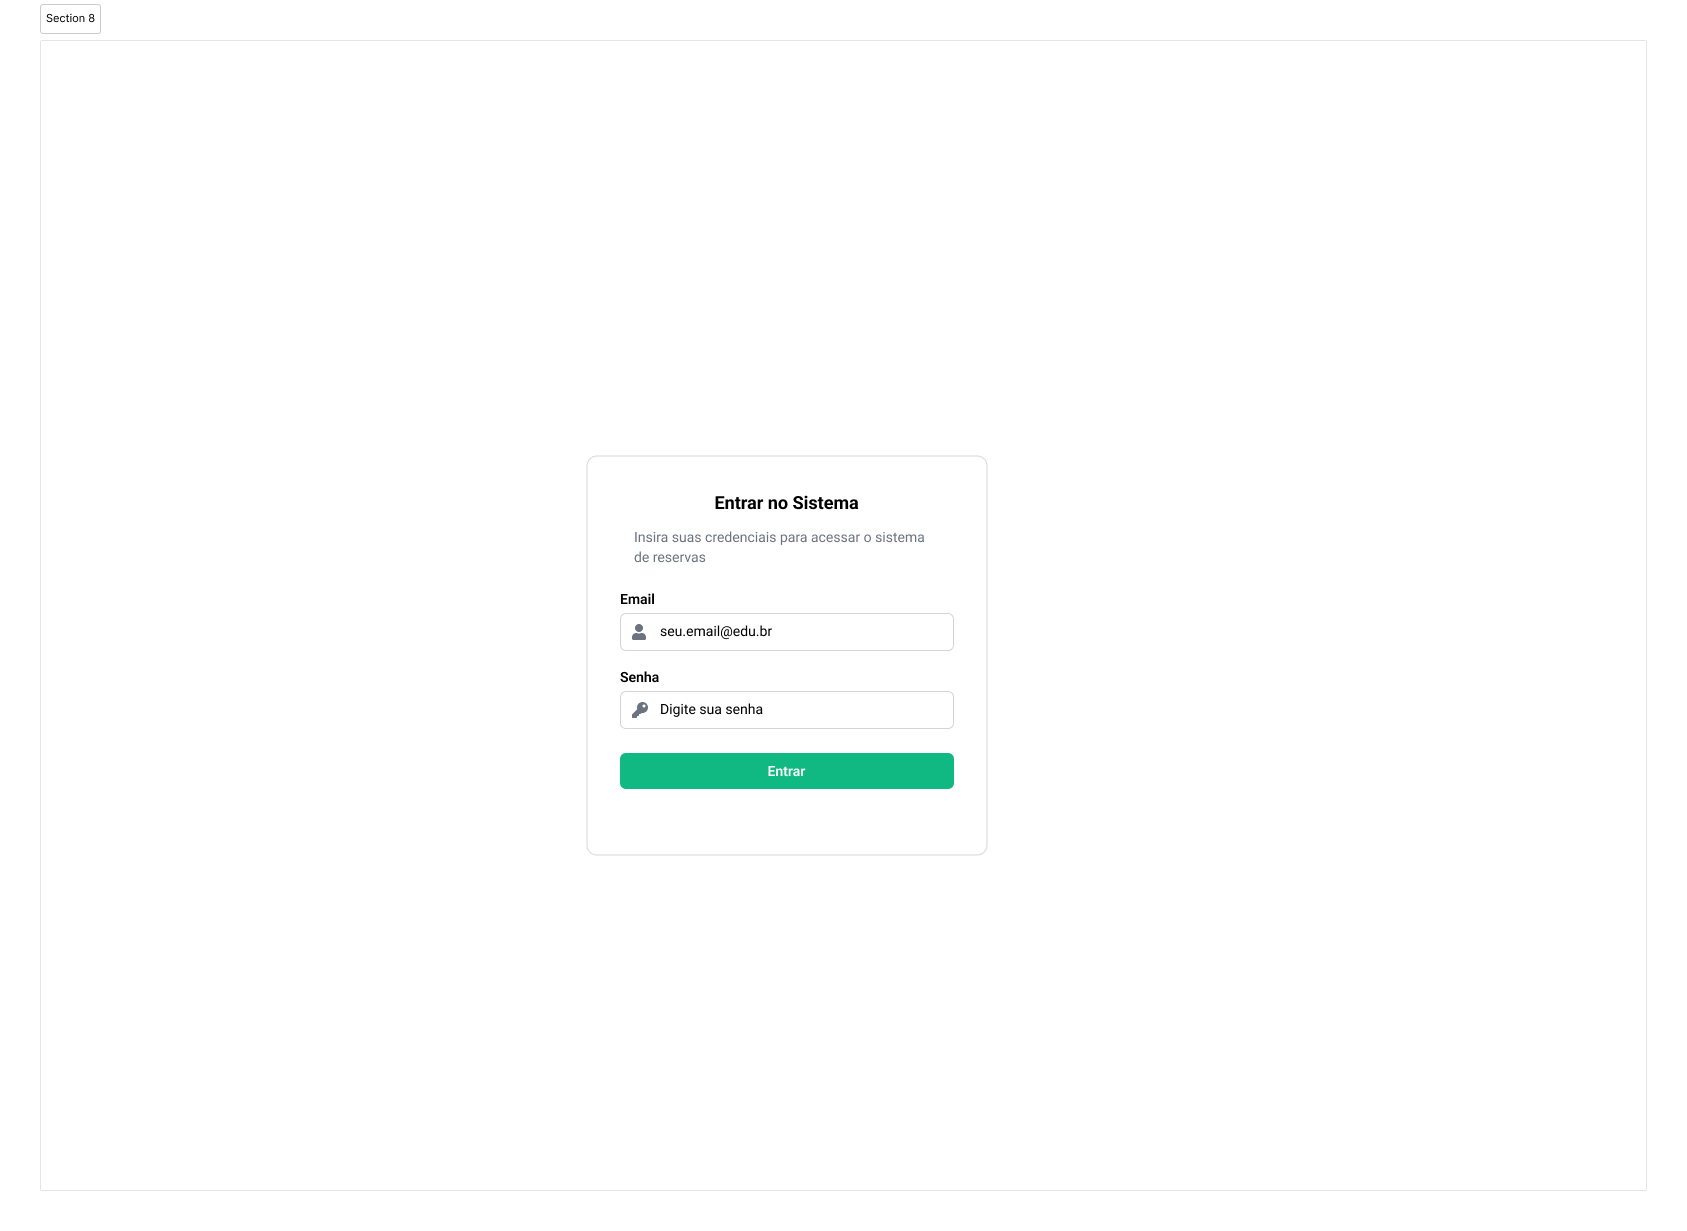
\includegraphics[width=\textwidth,height=0.72\textheight,keepaspectratio]{../relatorio-estagio/imagens/telas/login.png}
\caption{Autenticação com e-mail e senha}
\end{figure}
\end{frame}

\begin{frame}
\frametitle{Gerenciamento de Salas}
\begin{figure}
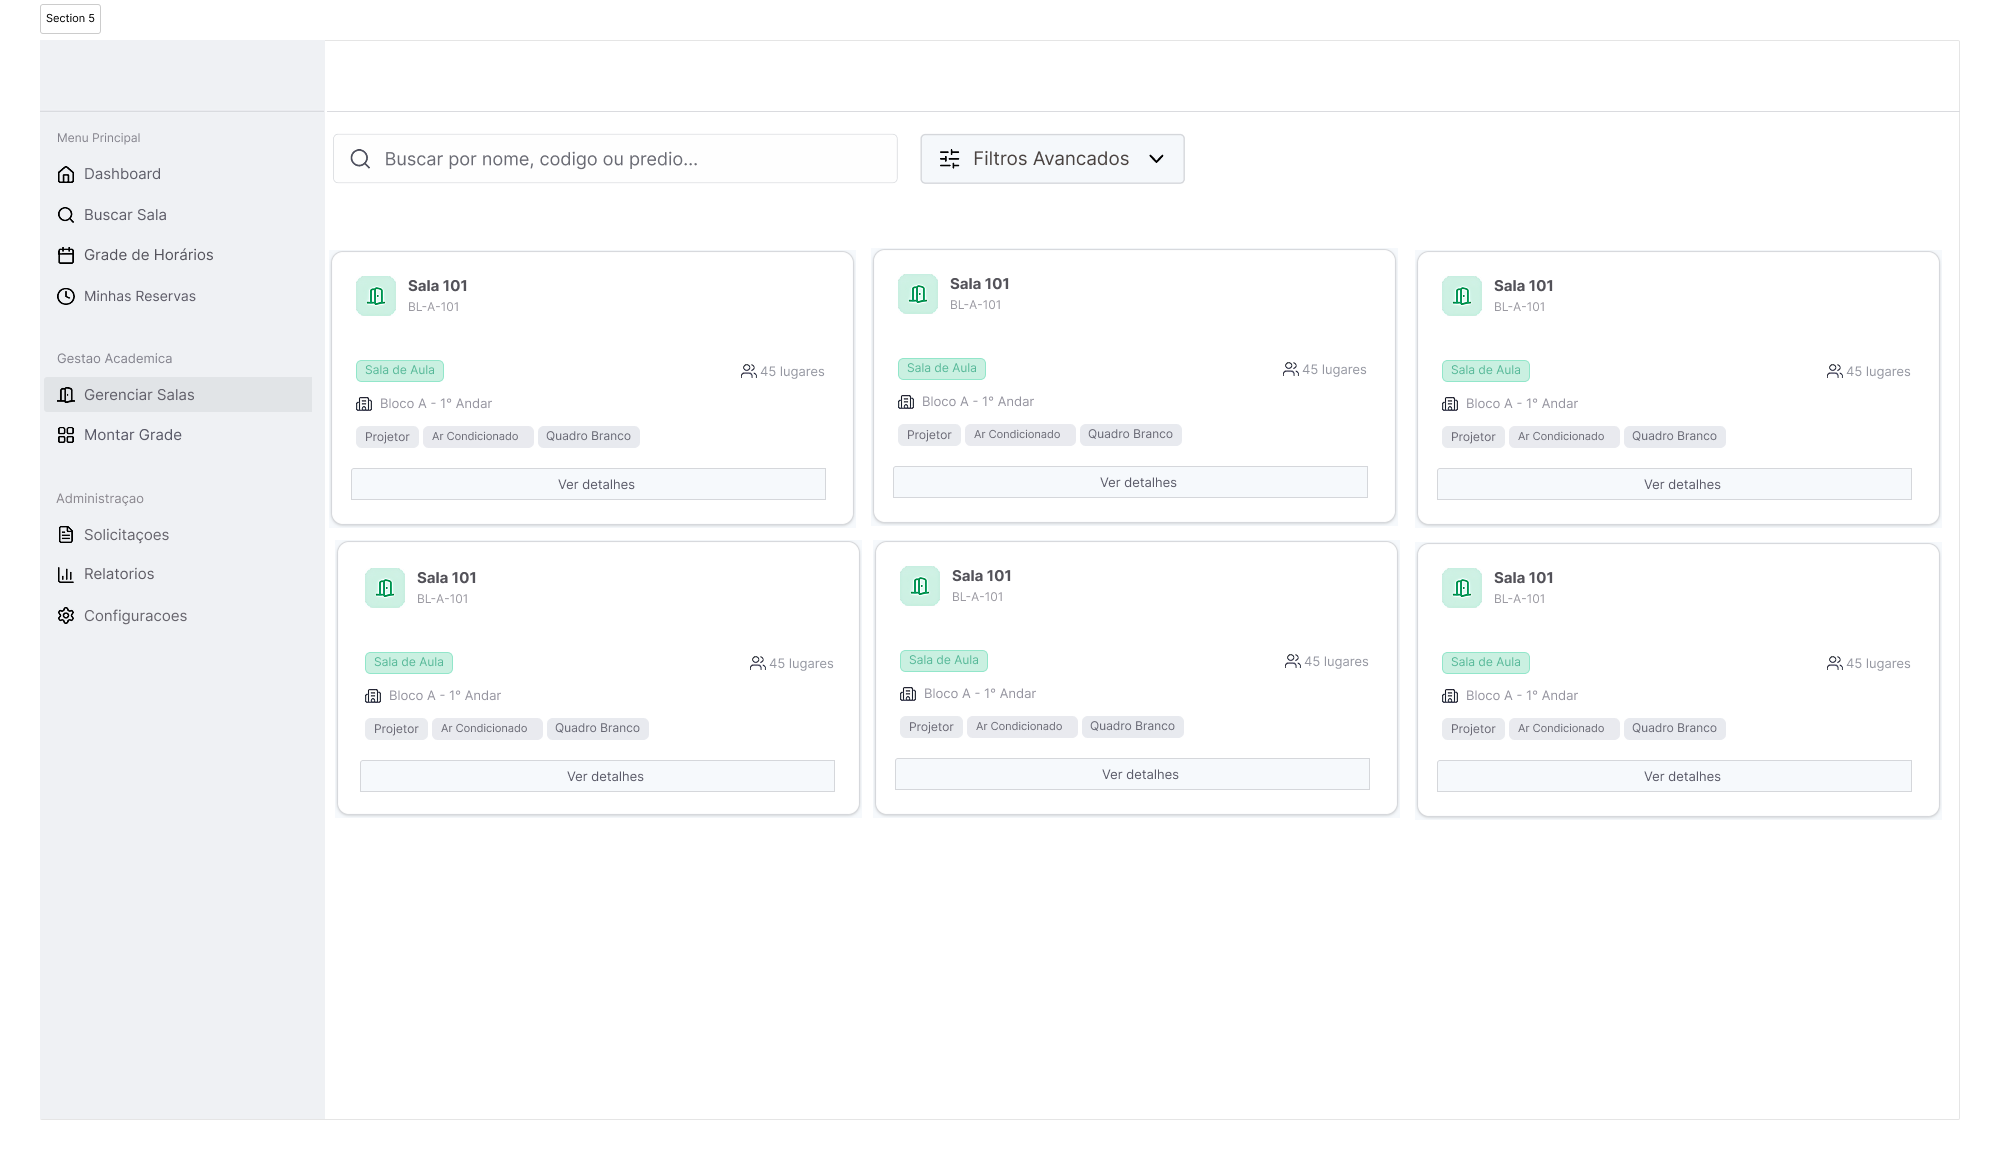
\includegraphics[width=\textwidth,height=0.72\textheight,keepaspectratio]{../relatorio-estagio/imagens/telas/gerenciar-salas.png}
\caption{Visualização, cadastro, edição e remoção de salas}
\end{figure}
\end{frame}

\begin{frame}
\frametitle{Buscar Sala}
\begin{figure}
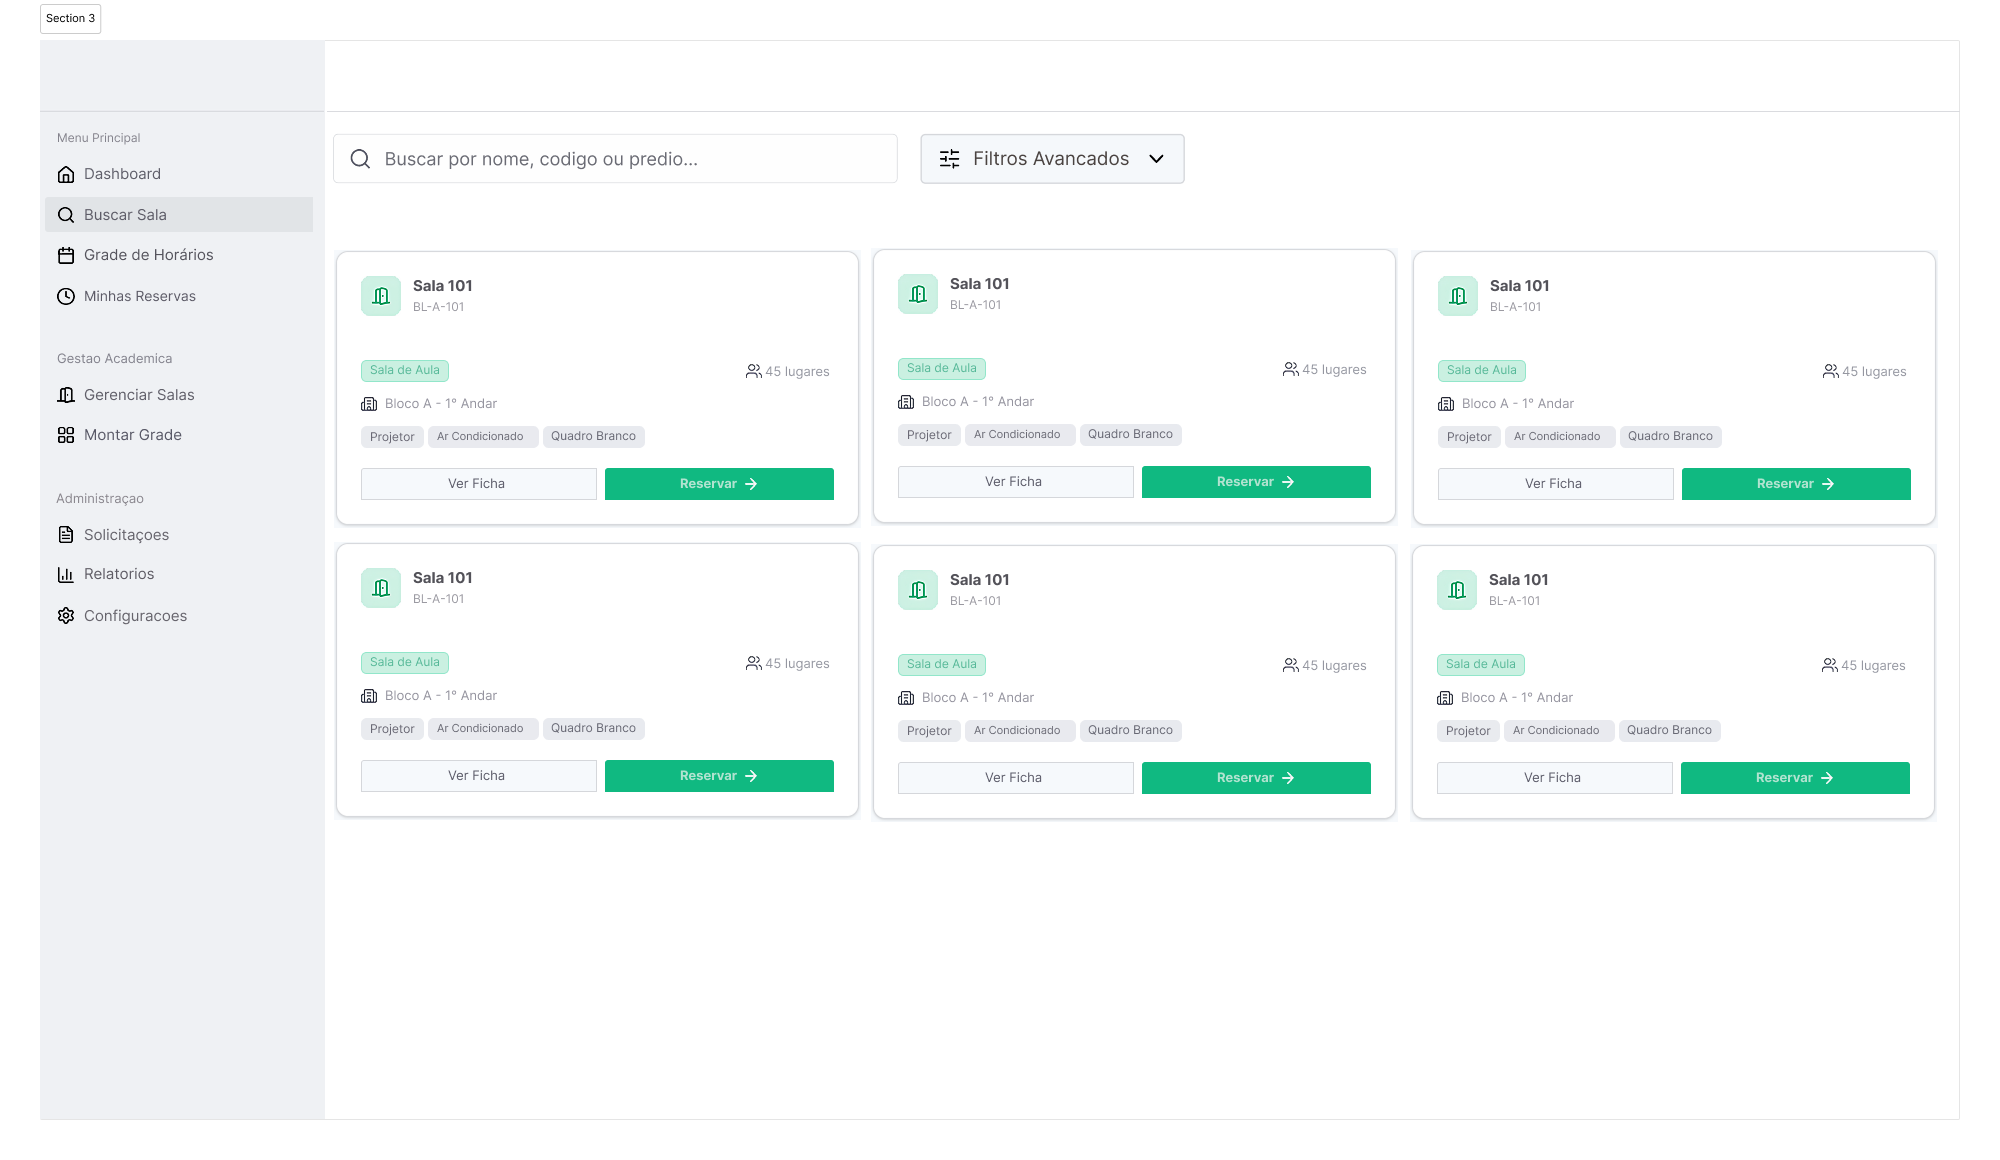
\includegraphics[width=\textwidth,height=0.72\textheight,keepaspectratio]{../relatorio-estagio/imagens/telas/buscar-sala.png}
\caption{Consulta de salas disponíveis}
\end{figure}
\end{frame}

\begin{frame}
\frametitle{Minhas Reservas}
\begin{figure}
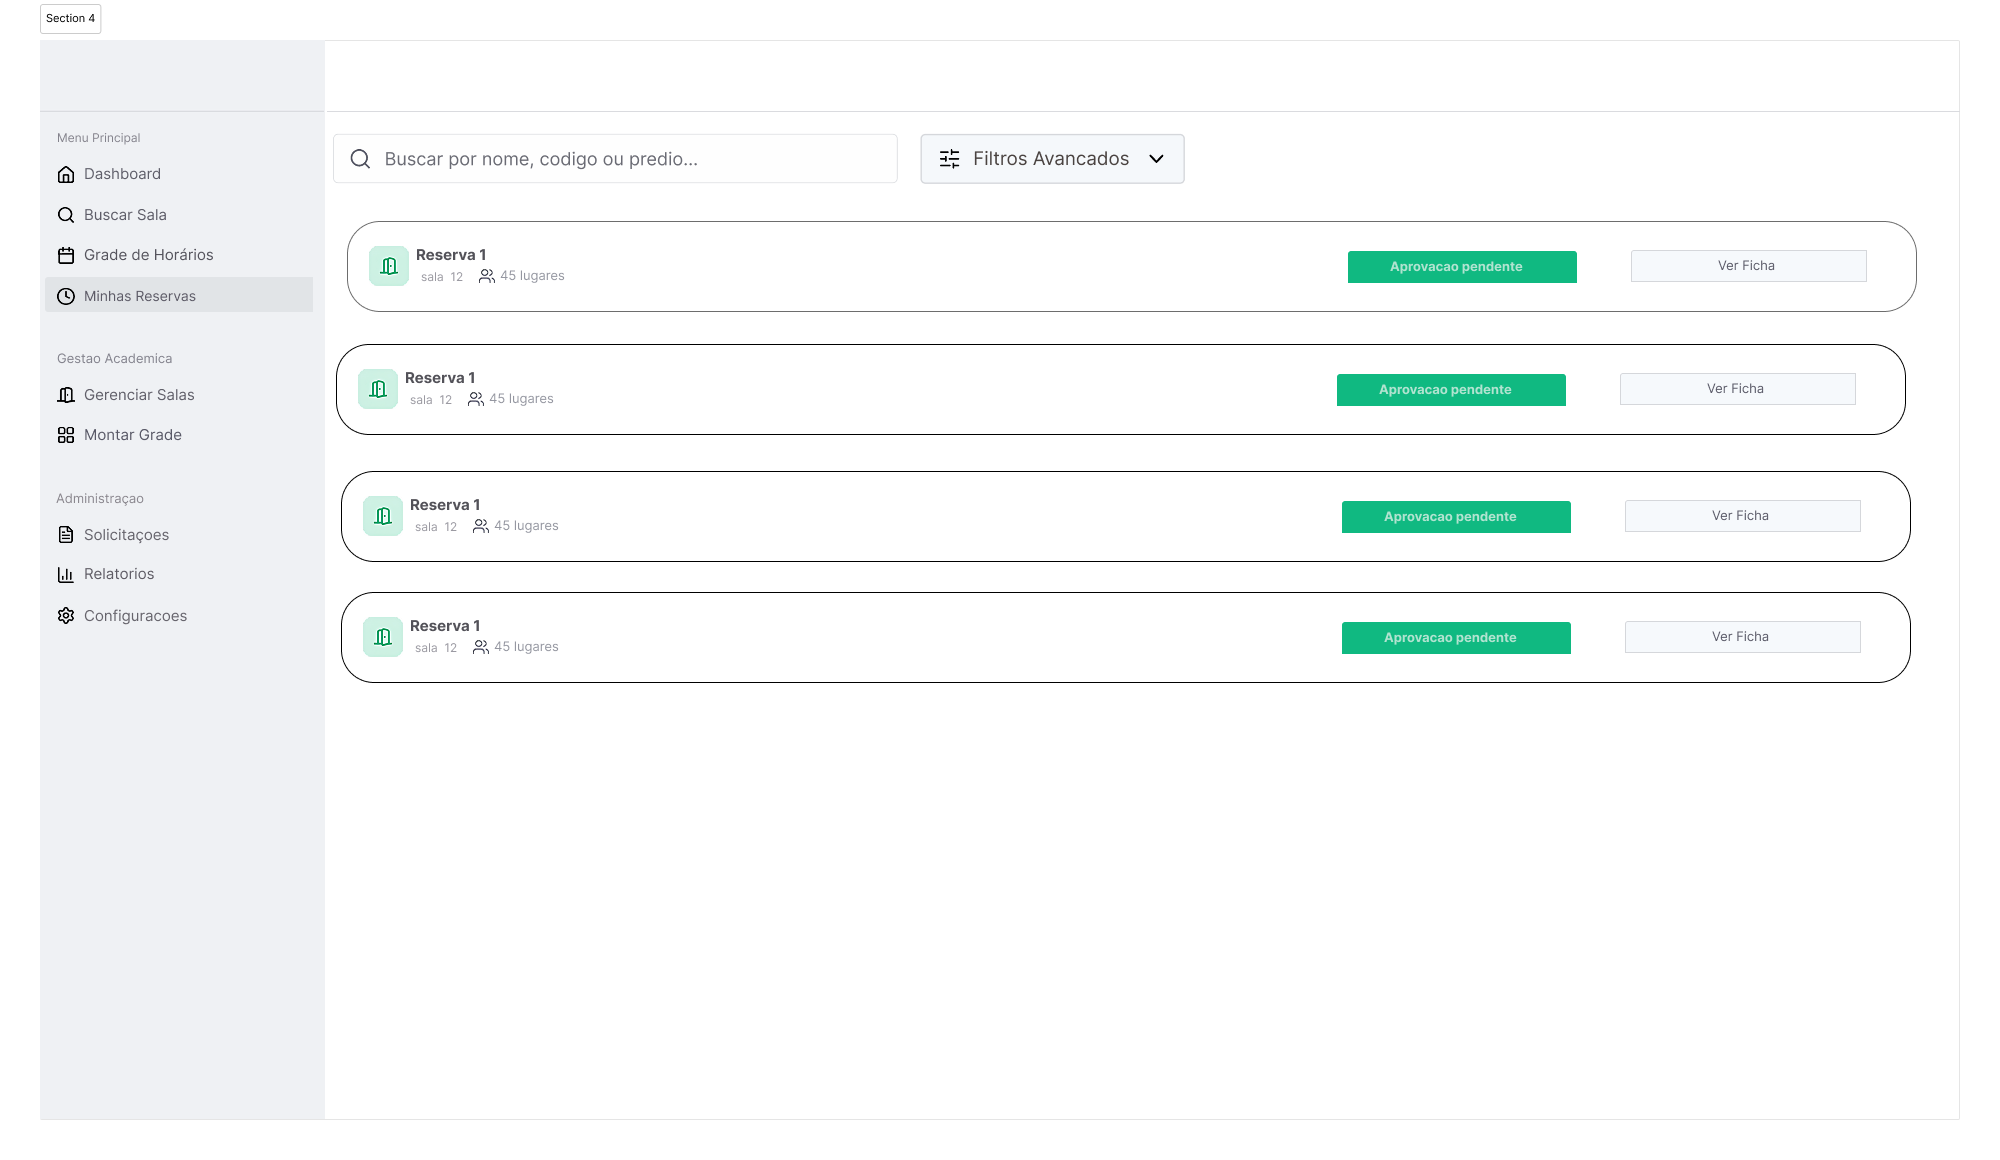
\includegraphics[width=\textwidth,height=0.72\textheight,keepaspectratio]{../relatorio-estagio/imagens/telas/minhas-reservas.png}
\caption{Acompanhamento dos agendamentos realizados}
\end{figure}
\end{frame}

\begin{frame}
\frametitle{Solicitações}
\begin{figure}
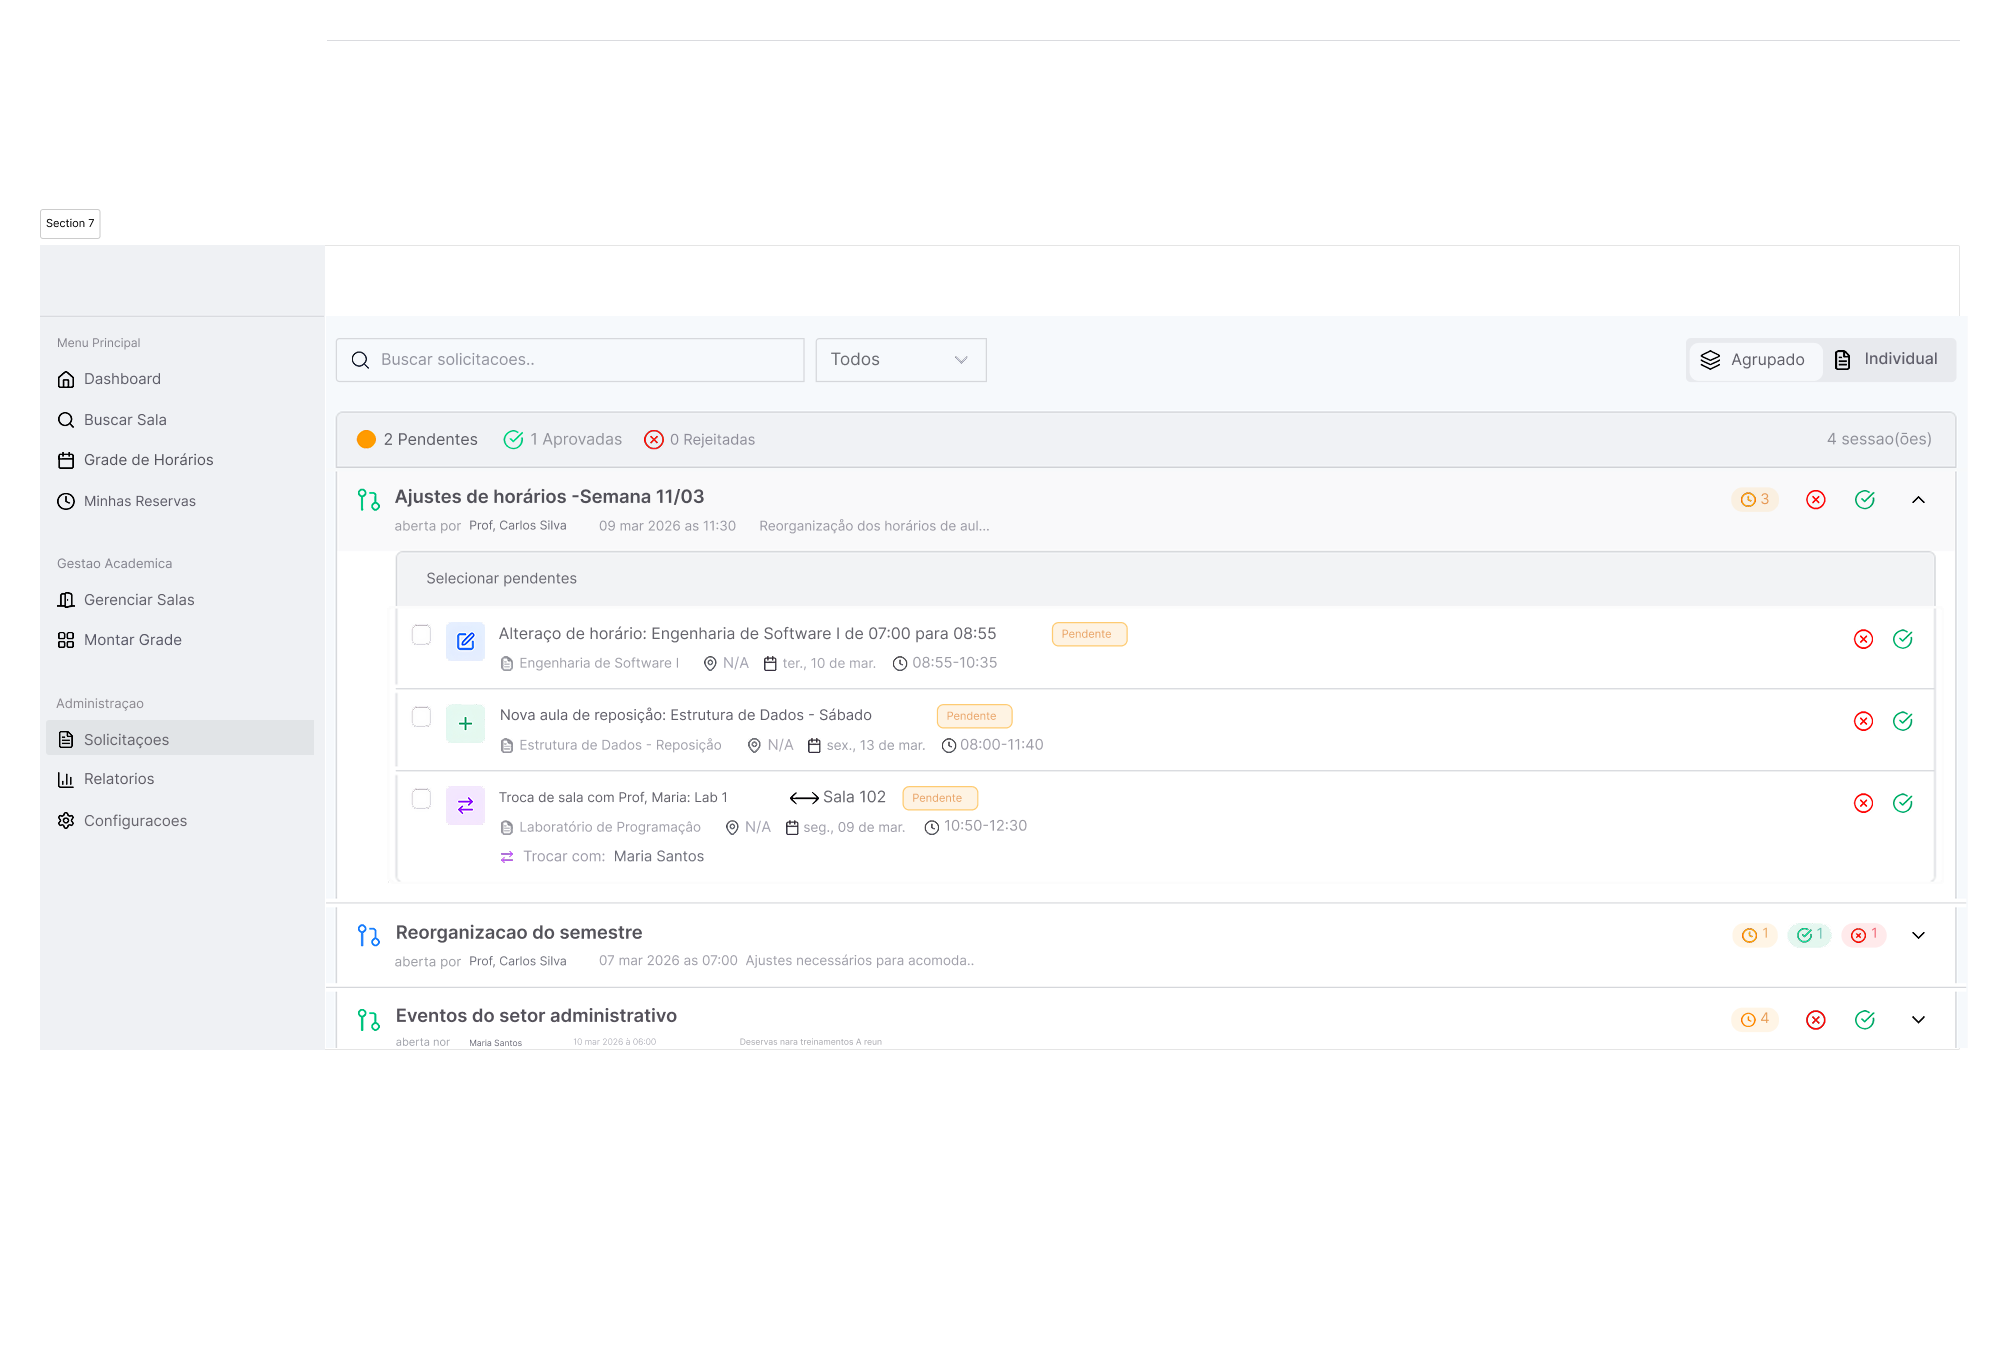
\includegraphics[width=\textwidth,height=0.72\textheight,keepaspectratio]{../relatorio-estagio/imagens/telas/solicitacoes.png}
\caption{Pedidos e seus respectivos status}
\end{figure}
\end{frame}

\begin{frame}
\frametitle{Grade de Horários}
\begin{figure}
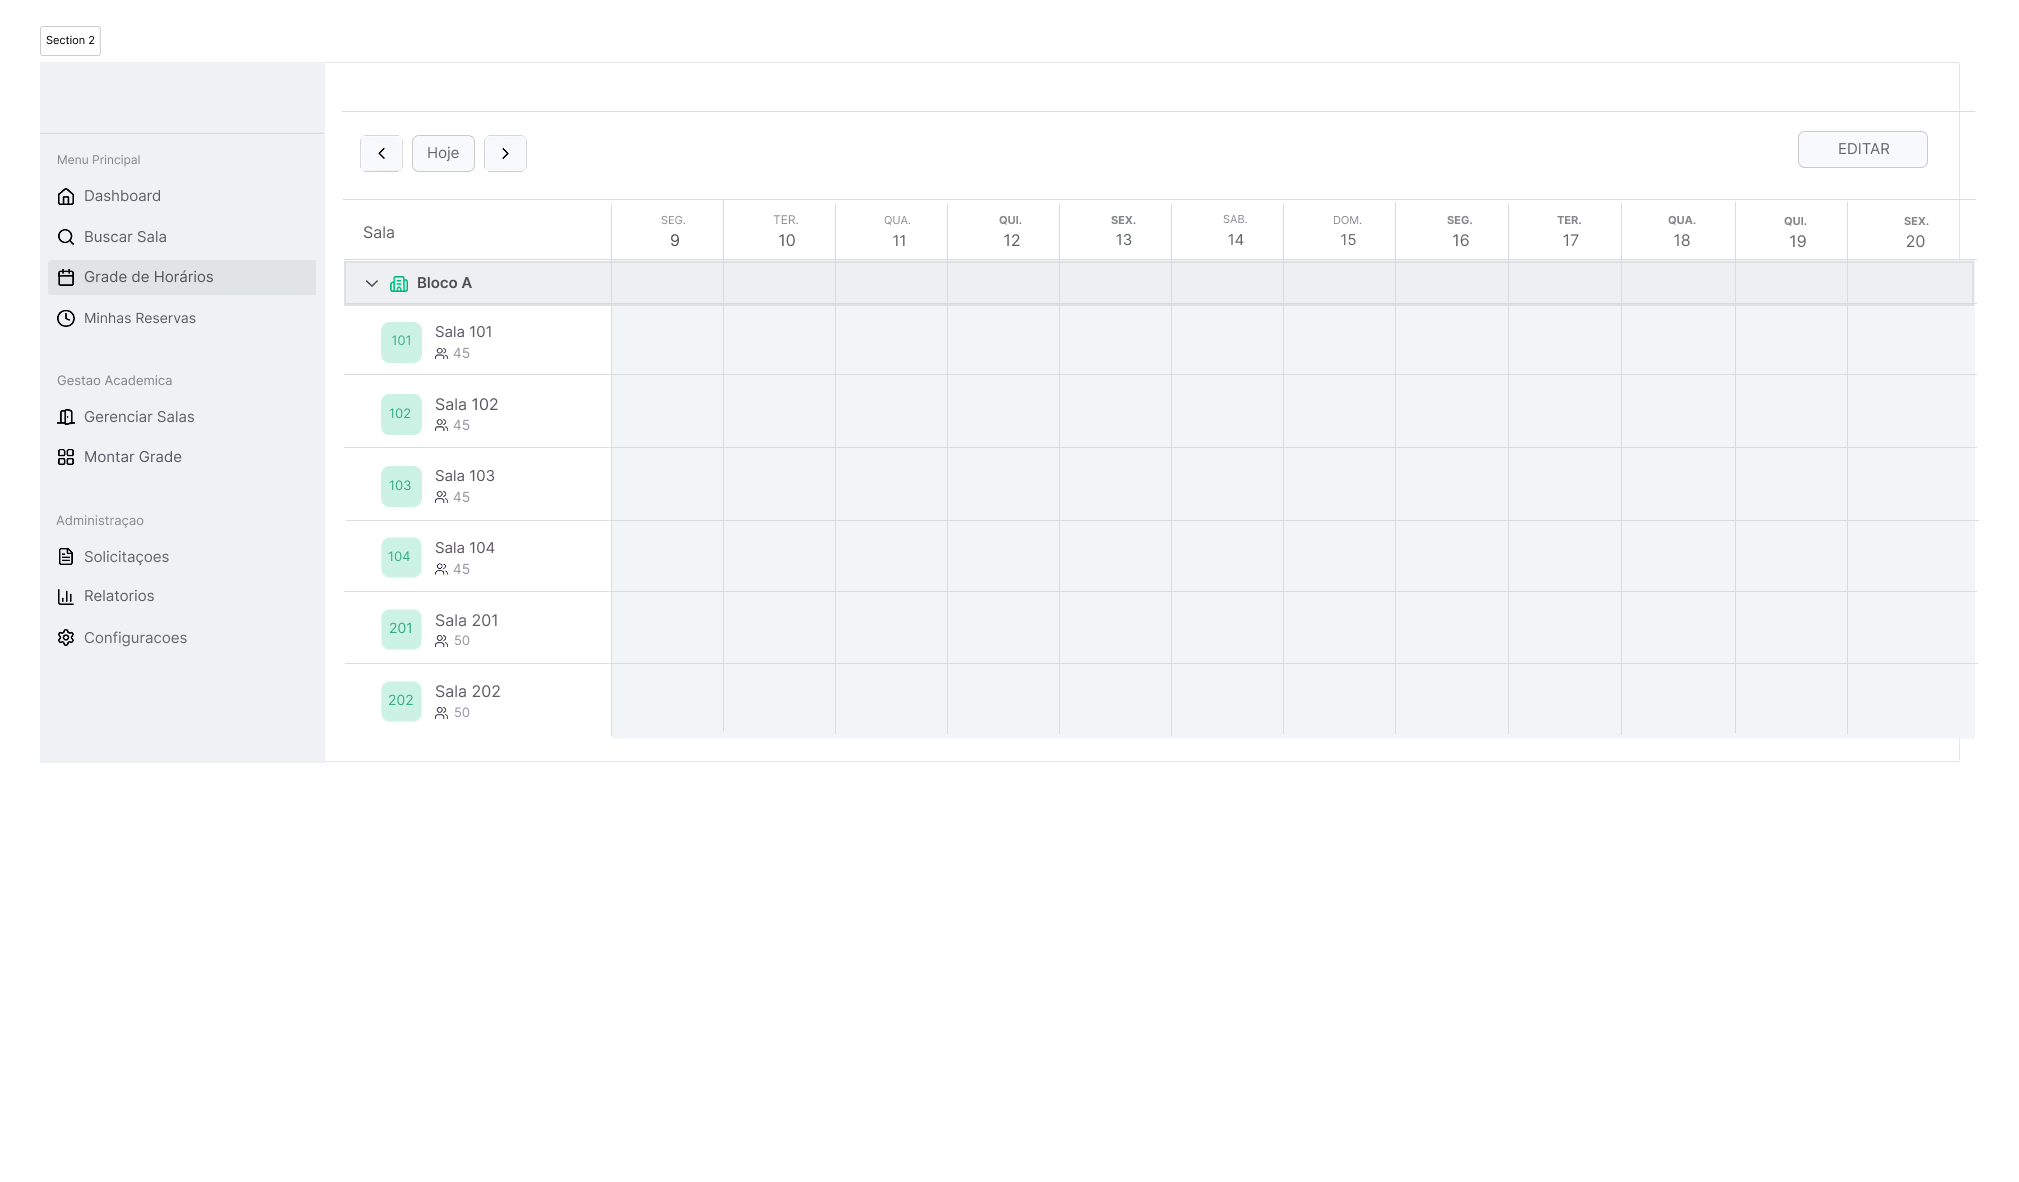
\includegraphics[width=\textwidth,height=0.72\textheight,keepaspectratio]{../relatorio-estagio/imagens/telas/grade-horarios.png}
\caption{Visualização da ocupação e disponibilidade das salas}
\end{figure}
\end{frame}

\begin{frame}
\frametitle{Montar Grade}
\begin{figure}
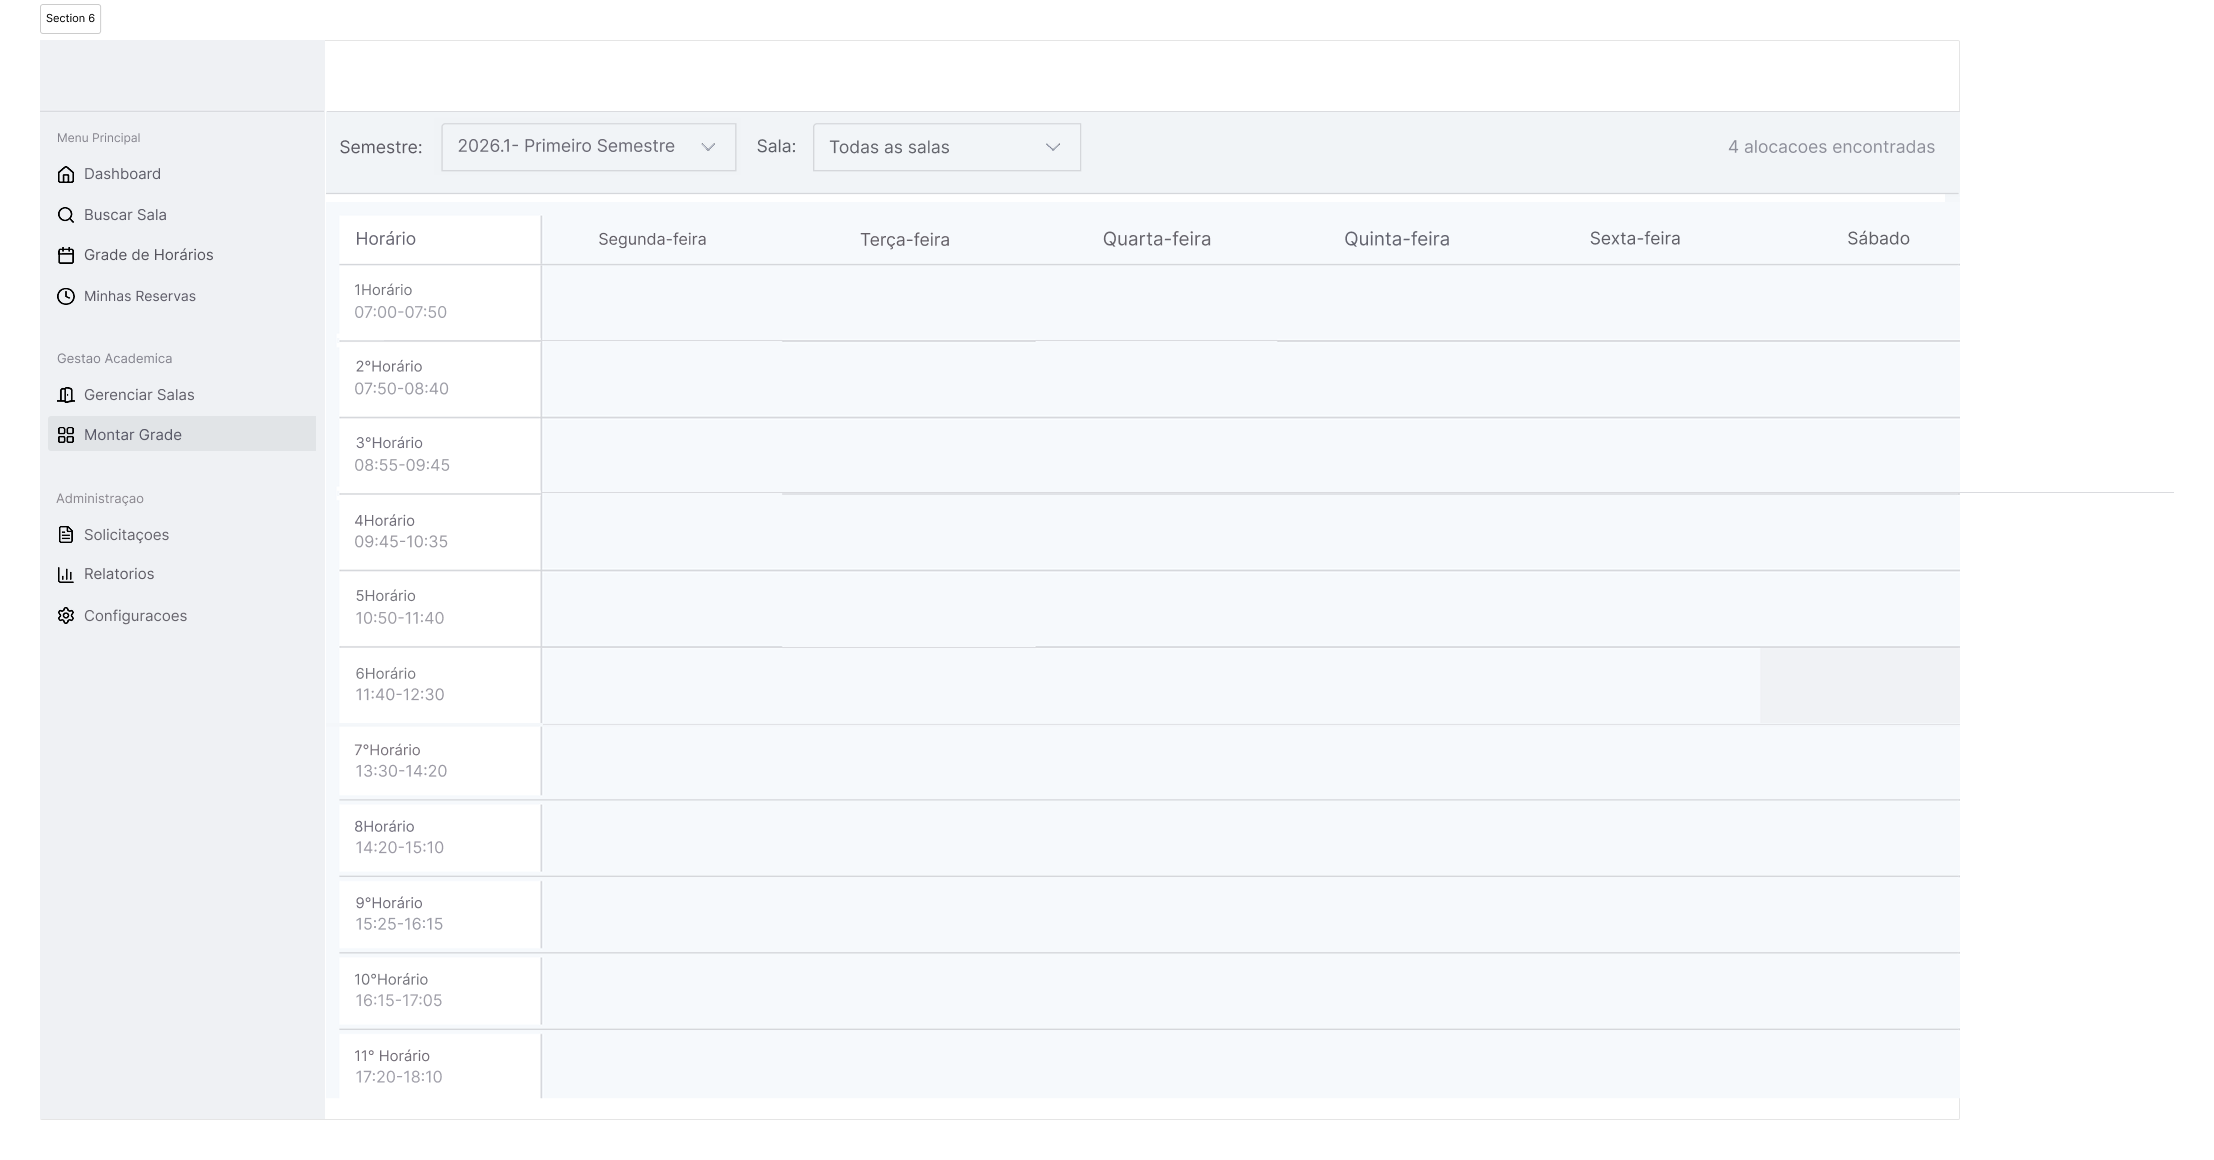
\includegraphics[width=\textwidth,height=0.72\textheight,keepaspectratio]{../relatorio-estagio/imagens/telas/montar-grade.png}
\caption{Estruturação da grade de horários por sala}
\end{figure}
\end{frame}

\lastslide

\end{document}
